\documentclass[tikz]{standalone}

% Pour le dégradé au centre du schéma
\usetikzlibrary{positioning, fadings}
% Permet d'importer des images et des graphiques.
\usepackage{graphicx}
\graphicspath{{./figures}} % chemin vers les figures


\begin{document}
\begin{tikzpicture}[>=stealth, thick, scale=0.75, every node/.style={scale=0.75}]
    \node[draw, circle, minimum width=1.25cm] (x0) {$x_0$};
    \node[draw, circle, minimum width=1.25cm, right=of x0] (x1) {$x_1$};
    \node[draw, circle, minimum width=1.25cm, right=of x1] (x2) {$x_2$};

    \node[right=of x2] (dots) {\dots};

    \node[draw, circle, minimum width=1.25cm, right=of dots] (xT1) {$x_{T-1}$};
    \node[draw, circle, minimum width=1.25cm, right=of xT1] (xT) {$x_T$};

    \node[above left=.2cm of x0] (cat) {
        
\includegraphics[width=1.5cm]{pure_cat_cifar10.png}
    };
    \node[below right=.2cm of xT] (noise) {
        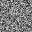
\includegraphics[width=1.5cm]{pure_gaussian_noise.png}
    };


    \draw[->] (x0) edge[bend left] node[above] {$q(x_1|x_0)$} (x1);
    \draw[->] (x1) edge[bend left] node[below] {$p(x_0|x_1)$} (x0);

    \draw[->] (x1) edge[bend left] node[above] {$q(x_2|x_1)$} (x2);
    \draw[->] (x2) edge[bend left] node[below] {$p(x_1|x_2)$} (x1);

    \draw[->] (x2) edge[bend left, path fading=east] (dots);
    \draw[->] (dots) edge[bend left, path fading=east] (x2);

    \draw[->] (dots) edge[bend left, path fading=west] (xT1);
    \draw[->] (xT1) edge[bend left, path fading=west] (dots);

    \draw[->] (xT1) edge[bend left] node[above] {$q(x_T|x_{T-1})$} (xT);
    \draw[->] (xT) edge[bend left] node[below] {$p(x_{T-1}|x_T)$} (xT1);

    \draw (cat) -- (x0);
    \draw (xT) -- (noise);
\end{tikzpicture}
\end{document}